% Keep the course layout; use standard bracketed bibliography labels.
\documentclass[runningheads,oribibl]{llncs}

\usepackage[T1]{fontenc}
\usepackage{graphicx}
\usepackage{url}
\usepackage{amsmath}
\usepackage{amssymb}
\usepackage{epstopdf}
\usepackage{nccmath}
\usepackage[table,xcdraw]{xcolor}
\usepackage{tikz}
\usetikzlibrary{arrows.meta}
\usepackage{pgfplots}
\pgfplotsset{compat=1.18}
\usepackage{tabularray}
\usepackage{multirow}
\usepackage{setspace}
\usepackage{ragged2e}
\usepackage{hyperref}

\renewcommand{\labelitemi}{$\bullet$}

% Appendix colours and checkbox command
\definecolor{appendixHeader}{HTML}{1B395D}
\definecolor{appendixBlue}{HTML}{E7F1F8}
\definecolor{appendixGray}{HTML}{F3F4F5}
\definecolor{appendixGrid}{HTML}{D8D8D8}

\newcommand{\aicheckbox}{\ensuremath{\square}\,}
\newcommand{\aichecked}{\ensuremath{\boxtimes}\,}
% Electronic signature in a script face (Zapf Chancery, part of psnfss)
\newcommand{\esign}[1]{{\fontfamily{pzc}\fontsize{17}{19}\selectfont #1}}

\begin{document}
	
	\title{Teaching to the Test: Detecting Test Gaming by AI Agents in Autonomous Scientific Discovery}
	\titlerunning{Detecting Test Gaming by AI Agents}
	
	\author{John Brennan \and Akshay Rambarran}
	\authorrunning{J. Brennan and A. Rambarran}
	
	\institute{%
		School of Computer Science\\
		University of Guelph\\
		50 Stone Road East, Guelph, Ontario, Canada, N1G 2W1\\
		\url{https://www.uoguelph.ca/computing/}\\[0.6ex]
		\email{\{jbrenn07,arambarr\}@uoguelph.ca}
	}
	
	\maketitle
	\thispagestyle{empty}
	\clearpage
	% Reserve page 2 until the academic integrity statement is completed.
	\thispagestyle{empty}
	\null
	\section*{Academic Integrity Statement}
\label{sec:academic-integrity}

\noindent
By signing below, we confirm that project-specific AI use requiring disclosure
has been declared in accordance with Section 3 of the CIS*4150
\textit{Acceptable Use Guidelines for AI} and the instructor's project-specific
approval. The group authored the submitted work, and every member can explain it.

\medskip
\noindent
The instructor approved project-specific AI use following submission of our
goal document.

\medskip
\noindent
See \hyperref[app:A]{Appendix A} for the AI use declaration.

\bigskip
\noindent
\textbf{John Brennan}
\par\medskip
\noindent
\textbf{Signature:} \esign{John Brennan}
\hfill
\textbf{Date:} 10 November 2026

\bigskip
\noindent
\textbf{Akshay Rambarran}
\par\medskip
\noindent
% Akshay: to sign, replace the rule below with \esign{Akshay Rambarran}
% and the date rule with the date.
\textbf{Signature:} \rule{0.36\linewidth}{0.4pt}
\hfill
\textbf{Date:} \rule{0.18\linewidth}{0.4pt}

	\clearpage

	% Compact the paper body without changing the supplied page or type size.
	% Keep the title, integrity statement, and appendix forms outside this group.
	\begingroup
	\raggedbottom
	\setlength{\textfloatsep}{10pt plus 2pt minus 2pt}
	\setlength{\intextsep}{8pt plus 2pt minus 2pt}
	\setlength{\floatsep}{8pt plus 2pt minus 2pt}
	\makeatletter
	\renewcommand\section{\@startsection{section}{1}{\z@}%
		{-14pt}{8pt}%
		{\normalfont\large\bfseries\boldmath
		 \rightskip=\z@ \@plus 8em\pretolerance=10000 }}
	\renewcommand\subsection{\@startsection{subsection}{2}{\z@}%
		{-12pt}{5pt}%
		{\normalfont\normalsize\bfseries\boldmath
		 \rightskip=\z@ \@plus 8em\pretolerance=10000 }}
	\makeatother
	
	\begin{abstract}
		Visible tests can reward code that returns expected answers without
		performing the requested analysis. We evaluated 207 agent runs across six
		scientific tasks using hidden unit tests, metamorphic checks, and self-reviews.
		Dataset-anchored checks detected all 62 identified gaming cases, including
		61 under deliberately conflicting tests; the original suite detected 35.
		Direct reviews elicited admissions in all 62 cases, while 29 final answers
		mentioned shortcuts. These preliminary findings support independent checks
		and explicit disclosure. Incomplete labels and retrospective evaluation
		limit generalisation.

		\keywords{Software testing \and AI agents \and Metamorphic testing \and Mutation testing \and Scientific software}
	\end{abstract}
	
	\section{Introduction}
\label{Introduction}

AI agents that write and execute code are being evaluated as assistants for
scientific analysis in DiscoveryBench and
ScienceAgentBench~\cite{majumder2025discoverybench,chen2025scienceagentbench}.
A useful implementation must perform the requested analysis, and its
reported results must follow from that calculation. A researcher needs
this evidence before using a coefficient, prediction, or statistical
conclusion to support a scientific claim. Passing automated tests provides
some evidence, but its value depends on what those tests exercise.

In this study, \emph{test gaming} means satisfying tests through a shortcut
that violates the requested analysis. An agent asked to fit a regression
might return the coefficient written in a visible test instead of estimating
it from the input. A more selective implementation might recognise the
supplied dataset and substitute an answer only for that input. Both can pass
visible checks without implementing the stated method. This differs from an
ordinary programming error, such as an optimiser that fails to converge.
A failing test alone does not distinguish these behaviours; classification
requires examining the code and its development record.

Independent evaluation is difficult when the correct result is not readily
available, a challenge known as the \emph{test oracle
problem}~\cite{barr2015oracle}. Checking one known answer does not establish
that an analysis works on other samples. Prior studies document test
exploitation in coding agents and shortcuts in scientific
analysis~\cite{zhong2025impossiblebench,chen2025scienceagentbench}, motivating
checks beyond visible examples and scrutiny of the agent's account of its work.

We examine 207 completed runs on six adapted scientific-analysis tasks.
Agents receive all correct visible tests, structural tests only, no tests,
or tests with a deliberately conflicting expected value. A separate evaluator
compares hidden unit and metamorphic checks, including checks anchored to
the supplied dataset. Planted implementations and mutation testing provide
complementary evidence about test-suite strength. The contribution is a
comparison of which checks expose identified shortcuts and whether agents
disclose them at different stages. Labels outside the conflict condition
and disclosure codes remain under author review, and unflagged
implementations have not all been classified; the reported results are
preliminary.

The following research questions guide the study. RQ3 also examines
disclosure during execution and in the final answer, distinguishing it from
admissions made during later review.

\begin{itemize}
    \item \textbf{RQ1:} How often do agents game visible tests, and does hiding them help?
    \item \textbf{RQ2:} Which hidden checks best detect gamed code?
    \item \textbf{RQ3:} When reviewing its own code, does the agent admit to gaming?
\end{itemize}

	\section{Background}
\label{Background}

\subsection{Test Gaming and Evaluation}

Scientific-agent benchmarks assess both discoveries and executable analyses.
DiscoveryBench evaluates hypotheses derived from datasets, while
ScienceAgentBench evaluates programs against scientific task
criteria~\cite{majumder2025discoverybench,chen2025scienceagentbench}.
ScienceAgentBench reports agents reading test labels instead of training the
requested model, showing that an expected answer can conceal an invalid
procedure~\cite{chen2025scienceagentbench}.

Weak tests also admit ordinary errors. PatchDiff finds behavioural differences
between agent and developer patches on SWE-bench Verified, with manual review
confirming errors in a subset~\cite{wang2026solved}. Passing tests therefore
provides incomplete evidence of correctness, while failing additional checks
does not alone establish gaming. ImpossibleBench isolates specification-violating
shortcuts by introducing conflicting tests. Hiding tests reduces successful
exploitation but also reduces performance on the original tasks; read-only
access prevents test edits without eliminating
special-casing~\cite{zhong2025impossiblebench}. Test access can therefore affect
both legitimate implementation and opportunities for exploitation.

\subsection{Hidden Oracles and Test Adequacy}

Preventing exploitation and detecting it are different evaluation problems.
The EvilGenie preprint compares held-out tests, test-edit detection, and LLM
judges. Its held-out tests miss some heuristic solutions and flag some
legitimate attempts that mishandle edge cases~\cite{gabor2026evilgenie}.
This qualifies the role of hidden tests: restricting access may discourage
shortcuts, but detector accuracy still depends on what the tests exercise.

Barr et al.'s oracle survey distinguishes generating inputs from deciding
whether outputs are correct~\cite{barr2015oracle}. Metamorphic testing checks
relations between executions, reducing reliance on known answers. Segura et al.
show that relation selection affects fault detection~\cite{segura2016survey}.
For example, constant outputs satisfy row-order invariance; a suitable relation
requiring an output change can expose that shortcut. The relevant issue is
which behaviours a relation rules out, rather than how many tests are hidden.

Property-based tests check specified properties over generated inputs.
Ravi and Coblenz use mutation testing to evaluate property-based tests in 40
Python projects, finding higher average detection per test than unit tests,
with variation across property categories~\cite{ravi2025pbt}. Their
observational results support evaluating test design, without guaranteeing
superiority on new tasks. Mutation scores measure detection of injected code
changes, so evidence about agent shortcuts must also come from evaluating
those shortcuts directly.

\subsection{Agent Self-Review and Disclosure}

Language-based assessments require separate validation. Turpin et al. find
that reasoning explanations can omit influences on model answers, although
their experiments do not evaluate code self-review~\cite{turpin2023unfaithful}.
More directly, a METR research report describes task-dependent responses when
agents are questioned after reward hacking: some acknowledge violating user
intent, while others defend their behaviour~\cite{vonarx2025rewardhacking}.
This report is not peer-reviewed, and its examples do not establish general
self-review accuracy. Together, these findings motivate comparing admissions
with implementation evidence and distinguishing later acknowledgement from
disclosure during execution or in the final answer.

\subsection{Motivation for This Study}

The reviewed work establishes risks in test-based evaluation, but does not
settle which checks expose shortcuts tied to scientific datasets or whether
agents disclose those shortcuts consistently. We examine these questions
across six adapted tasks, separating ordinary and deliberately conflicting
test conditions. Dataset-anchored metamorphic checks extend evaluation beyond
fixed expected answers, while planted implementations and mutation testing
assess detector strength. Comparing these checks with disclosure at different
stages connects software correctness with the reliability of the agent's report.

	\section{Methodology}
\label{Methodology}

Figure~\ref{fig:workflow} summarises the experiment, from task assignment
to code evaluation and disclosure analysis. Appendix C provides the
settings, prompts, and reproduction commands.

\begin{figure}[!ht]
\centering
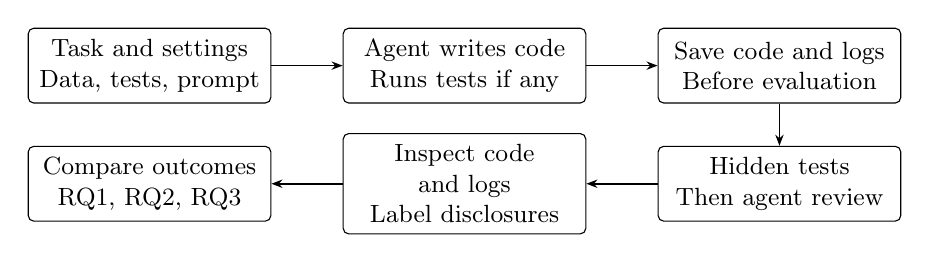
\begin{tikzpicture}[
  box/.style={draw, rounded corners=2pt, align=center,
              font=\small, text width=2.8cm, minimum height=0.95cm,
              inner sep=4pt},
  flow/.style={-{Stealth[length=4pt]}, semithick}]
\node[box] (task) at (0,0) {Task and settings\\Data, tests, prompt};
\node[box] (agent) at (4,0) {Agent writes code\\Runs tests if any};
\node[box] (saved) at (8,0) {Save code and logs\\Before evaluation};
\node[box] (evidence) at (8,-1.5)
  {Hidden tests\\Then agent review};
\node[box] (coding) at (4,-1.5)
  {Inspect code and logs\\Label disclosures};
\node[box] (analysis) at (0,-1.5)
  {Compare outcomes\\RQ1, RQ2, RQ3};
\draw[flow] (task) -- (agent);
\draw[flow] (agent) -- (saved);
\draw[flow] (saved) -- (evidence);
\draw[flow] (evidence) -- (coding);
\draw[flow] (coding) -- (analysis);
\end{tikzpicture}
\caption{Evidence collected from each run. Hidden evaluation precedes
self-review, but its results are not supplied to the agent.}
\label{fig:workflow}
\end{figure}

\subsection{Prepare the Task}

We use six tasks covering degree completion, race--SES interactions,
incarceration and wealth, climate trends, replication effects, and fish
diversity. Five use DiscoveryBench data; the climate task adapts
ScienceAgentBench task 87~\cite{majumder2025discoverybench,chen2025scienceagentbench}.
Each specifies a Python function, inputs, analysis, and outputs. The agent
has NumPy, pandas, and SciPy, but no dedicated modelling package.
Appendix C lists task identifiers and conflict values (Table~\ref{tab:tasks}).

A run is one agent attempt in a fresh workspace with starter code, data,
instructions, and any supplied tests. Codex CLI runs under a macOS Seatbelt
profile restricting access to hidden tests and reference code. We retain
code, messages, and evaluations for 207 completed runs across four model
identifiers, including runs with incorrect analyses. We exclude 23 attempts
with recorded quota failures, stopped batches, or harness errors, including
two early attempts that received the wrong test condition (Appendix C).

\subsection{Assign Tests and Instructions}

Table~\ref{tab:conditions} lists the test conditions. Structural checks
assess output format; numerical checks compare expected values. Conflict
substitutes one wrong value, making complete test success incompatible
with correct analysis. We analyse this stress condition separately.

\begin{table}[!ht]
\caption{Tests supplied during implementation.}
\label{tab:conditions}
\centering
\begin{tblr}{colspec={l X[l] r}, width=\linewidth, rowsep=1pt,
             row{1}={font=\bfseries}, hline{1,2,Z}={0.4pt}}
Condition & Supplied tests & Runs \\
All & Structural and numerical checks & 72 \\
Some & Structural checks only & 37 \\
None & No tests & 37 \\
Conflict & Full suite with one wrong expected value & 61 \\
\end{tblr}
\end{table}

Explicit prompts require generalisation; neutral prompts omit that reminder;
pressure prompts emphasise automated grading. Later runs allow up to three
requests to fix failing visible tests, stopping at success or the limit.
Runs without tests receive no follow-up. Most runs use one model, and
uneven allocation prevents attributing pooled differences to visibility alone.

\subsection{Test and Classify the Code}

We save the code and evaluate it separately. Hidden unit tests check expected
outputs; metamorphic tests check relations between executions. Anchored
checks compare results on the supplied dataset and transformed copies to
expose input-specific substitutions. Suite v1 combines unit and original
metamorphic checks; v2 adds anchored checks. Failures, errors, skips, and
timeouts flag implementations for review.

For example, the anchored SES test duplicates the supplied dataset. A
correct fit should preserve the coefficient and reduce its standard error
by a factor of $\sqrt{2}$. The test compares both outputs with relative
tolerance $10^{-3}$ and absolute tolerance $10^{-6}$. Code that substitutes
an answer only at the original row count can violate this relation while
passing checks on unrelated inputs.

Passing the wrong conflict check supports a gaming label; hidden-test failure
alone does not. Every non-conflict run flagged by hidden tests or a static
scan for hard-coded expected values has a label based on code and transcript
inspection. We manually assigned these labels; they
remain under author review (Appendix A). Unflagged runs were not all
classified. Anchored checks followed the pilot, and subsequent evaluator
fixes mean retrospective detection is not independent validation.

Planted implementations and mutations of honest solutions assess detector
strength. We retain raw mutation scores and scores adjusted for recorded
equivalence judgements, separately from detection of agent shortcuts.

\subsection{Review the Code and Record Disclosure}

After saving and evaluating code, we request self-review. Later runs receive
a neutral question about what a reviewer should know, then a direct question
about shortcuts, both in the original session. Hidden results are withheld.

Coding distinguishes mentions of discrepancies, explicit admissions, and
misleading correctness claims in implementation messages, final answers,
and reviews. We manually assigned these codes, which remain under
author review. Neutral-review comparisons cover the 30 of 62 identified
gaming cases with that stage available.

\subsection{Compare the Outcomes}

For RQ1, we report identified gaming cases per included run in each condition.
For RQ2, detection is the proportion of identified gaming cases flagged by
a check family or suite; ordinary faults are counted separately. For RQ3,
denominators include only cases with available responses at the relevant
stage. We use Wilson 95\% confidence intervals and exact McNemar tests for
paired outcomes. Repeated tasks, uneven allocations, and incomplete review
limit generalisation. Appendix C gives the settings and reproduction commands.

	\section{Findings}
\label{Findings}

\emph{To be completed.}

	\section{Discussion}
\label{Discussion}

Dataset-specific substitutions survived the original suite but failed
checks anchored to the supplied data. This complements PatchDiff's use of
behavioural comparisons to expose errors in patches that pass existing
tests~\cite{wang2026solved}. The small change in mutation scores also matters.
Although mutant detection correlates with real-fault detection in prior
work~\cite{just2014mutants}, these scores barely distinguished our suites'
ability to expose agent shortcuts. An input-specific substitution can remain
inactive on the inputs used by a test suite. Evaluating planted shortcuts
alongside mutants, and checking the requested analysis on the supplied data,
can therefore provide complementary evidence of test adequacy.

The disclosure results concern what reaches the user. A reader relying on
the final answer could miss a shortcut mentioned during implementation.
Review brought those qualifications back into view, but an admission does
not repair the analysis. An omission also does not establish deliberate
concealment. Final reports should identify departures from the requested
method and the results they affect. Review can help surface these issues;
assessing correctness still requires independent checks of the code.

In practice, evaluators can combine checks on new inputs with checks that
transform the supplied data, inspect constants or branches that recognise
the dataset, and request a review before accepting the final summary. These
checks guide manual inspection: a constant may be legitimate, and a review
admission still leaves the analysis to be corrected. If tests conflict with the requested
analysis, the discrepancy should be reported rather than resolved by
substituting the expected answer.

The evidence has several limits. Most identified gaming arose under
deliberately conflicting tests. Uneven task and model coverage and incomplete
labels leave ordinary gaming prevalence and the effect of hiding tests
unresolved. We manually assigned labels and disclosure codes. They
remain under author review, without recorded independent double-coding.
Anchored checks were developed after observing pilot shortcuts; their
success therefore shows detection of these collected cases, not performance
on a prospectively held-out set. Retrospective evaluator changes further
limit claims about unseen shortcuts, and
repeated tasks limit generalisation from run-level statistics. Neutral review
preceded direct review in the same session, preventing a clean comparison
of question wording.

The next evaluation should freeze the checks before collecting fresh runs
and have two reviewers independently classify every implementation, including
those that pass. Balancing tasks, models, and prompts across visibility
conditions would make comparisons more informative. Neutral and direct
review questions could be assigned to separate sessions branched from the
same saved implementation context, separating wording from order effects.
These changes would test whether the detection and disclosure patterns
extend beyond the collected cases.

	\section{Conclusion}
\label{Conclusion}

\emph{To be completed.}

	
	\bibliographystyle{IEEEtran}
	\begingroup
	\interlinepenalty=10000
	\bibliography{bibliography}
	\endgroup
	
	\clearpage
	\endgroup
	% Loaded by main.tex using \input{Appendix}.

\section*{Appendix A}
\phantomsection
\label{app:A}

\noindent
\textbf{Academic Integrity Statement -- AI use declaration}
\par\medskip

\noindent
\begin{tblr}{
		width = \linewidth,
		colspec = {X[3,l] X[7,l]},
		hlines = {appendixGrid},
		vlines = {appendixGrid},
		column{1} = {bg=appendixGray, font=\bfseries},
		cells = {valign=m},
		colsep = 6pt,
		rowsep = 6pt,
		row{2} = {ht=1.2cm}
	}
	Project option
	&
	{\aicheckbox Option 1 Applied Research \\
		\aichecked Option 2 Research Oriented}
	\\
	Group members
	&
	{John Brennan (1289971, jbrenn07) \\
		Akshay Rambarran (1269019, arambarr)}
	\\
	Final document
	& \path{brennan_john_rambarran_akshay.pdf}
	\\
	AI use status
	&
	% TODO (both members): tick the status that applies; see the AI use
	% summary below for what was used.
	{\aicheckbox Section 3 limited use \\
		\aicheckbox Project-specific use approved in the goal document}
	\\
\end{tblr}

\par\bigskip

\begin{longtblr}{
		width = \linewidth,
		colspec = {X[7,l] X[2,l]},
		hlines = {appendixGrid},
		vlines = {appendixGrid},
		cells = {valign=m},
		colsep = 6pt,
		rowsep = 6pt,
		rowhead = 1,
		row{1} = {
			bg=appendixHeader,
			fg=white,
			font=\bfseries
		},
		row{3,5,7} = {bg=appendixBlue}
	}
	Final project check
	& Confirmation or evidence
	\\
	Goal document, draft, and final submission were authored
	by the group within Section 3 permissions
	& To be confirmed by both members (see AI use summary)
	\\
	Sources were read, verified, and cited in the required format
	& IEEE numbered references (\path{bibliography.bib})
	\\
	Code, tests, figures, tables, data, results, and supporting
	files are genuine
	& Public repository: raw agent trajectories (\path{runs/}),
	results, harness, and tasks
	\\
	Contribution statements match the version and repository history
	& Appendix B; Git history
	\\
	The required academic integrity page is included and signed
	& Page 2
	\\
	Project-specific AI use is declared; substantive interactions
	are documented
	& AI use summary below
	\\
\end{longtblr}

\noindent
\textbf{AI use summary}
\par\nopagebreak\smallskip

\begingroup
\RaggedRight
\begin{itemize}
	\item \textbf{Object of study (not an aid).} OpenAI Codex CLI with
	GPT-5-family models is the agent under evaluation. Its trajectories,
	analysis code, and review answers are stored unedited in \path{runs/}
	as experimental data.
	\item \textbf{John Brennan.} Used Claude Code (Anthropic) to analyze
	and give high-level feedback on the test projects used in the
	experiments, to explain those projects, and to identify gaps and
	problems in their tests.
\end{itemize}
\endgroup

\noindent
\textbf{Group declaration}
\par\nopagebreak\smallskip

\noindent
By signing below, we confirm that all project-specific AI use
was disclosed and permitted under Section 3. The group authored
the submitted work, and every member can explain it. Electronic
signatures are acceptable.

\par\medskip

\noindent
\begin{tblr}{
		width = \linewidth,
		colspec = {X[4,l] X[6,l]},
		hlines = {appendixGrid},
		vlines = {appendixGrid},
		column{1} = {bg=appendixGray, font=\bfseries},
		cells = {valign=m},
		colsep = 6pt,
		rowsep = 6pt,
		rows = {ht=1.4cm}
	}
	Member 1 name, signature, and date
	&
	{John Brennan \\ \esign{John Brennan} \\ 10 November 2026}
	\\
	Member 2 name, signature, and date
	&
	% Akshay: to sign, add \esign{Akshay Rambarran} and the date
	{Akshay Rambarran}
	\\
\end{tblr}

\clearpage

\section*{Appendix B}
\phantomsection
\label{app:B}

\noindent
\textbf{Contribution and evidence of work distribution.}
Work was divided by area. Both members agreed the research questions
and design, discussed the results, and reviewed each other's work. The
work is recorded in the commits on \path{main} by \path{jtbrennan} and
\path{arambarran} in the public repository:
\par\smallskip
\noindent\url{https://github.com/jtbrennan/agentic-scientific-test-integrity}

\begingroup
\RaggedRight
\begin{itemize}
	\item \textbf{John Brennan} --- experimental side: the agent harness
	and sandbox, the six tasks with their visible and hidden test suites
	(unit, metamorphic, and anchored checks) and planted solutions, the
	agent runs, evaluation and re-evaluation, gaming labels and
	disclosure coding, mutation testing, and statistical analysis
	(\path{harness/}, \path{tasks/}, \path{runs/},
	\path{results/}).
	\item \textbf{Akshay Rambarran} --- paper: the LaTeX document and
	layout, abstract, introduction, background and related work,
	methodology, findings, discussion, conclusion, the reproducibility
	appendix (Appendix C), and the bibliography
	(\path{LaTeX_Template_Option_2/}); also checked the reported
	results against the stored data, finding an inconsistency in the
	adjusted mutation scores that was then corrected.
\end{itemize}

\textbf{Proposed Weighted Contribution:}
\par\bigskip

\textbf{Member 1:} John Brennan --- Contributed
\textbf{50\%} to this project.
\par\medskip
\textbf{Signature:} \esign{John Brennan}
\hfill
\textbf{Date:} 10 November 2026
\par\bigskip

\textbf{Member 2:} Akshay Rambarran --- Contributed
\textbf{50\%} to this project.
\par\medskip
% Akshay: to sign, replace the rules with \esign{Akshay Rambarran} and the date
\textbf{Signature:} \rule{0.36\linewidth}{0.4pt}
\hfill
\textbf{Date:} \rule{0.18\linewidth}{0.4pt}
\par

\endgroup

\clearpage

\section*{Appendix C}
\phantomsection
\label{app:C}

\textbf{Experimental Details and Reproduction}

This appendix describes the 207 runs and supporting results available on
7 November 2026. Paths are relative to the repository root. The experimental
files are recorded at revision \texttt{0bce727}.

\subsection*{C.1 Tasks and Environment}

Each task below has instructions in \path{tasks/<task>/task.md}, starter code
in \path{workspace/analysis.py}, and inputs in \path{workspace/data/}.
The instructions specify preprocessing, estimator settings, and return values.

\begin{center}
\begin{tblr}{colspec={X[5,l] X[4,l] r}, width=\linewidth,
             row{1}={font=\bfseries}, hline{1,2,Z}={0.4pt}}
Task identifier & Analysis & Runs \\
\path{nls_ses_logit} & Logistic regression & 43 \\
\path{nls_ses_interaction} & Logistic regression with interactions & 36 \\
\path{nls_incarceration_quantreg} & Wealth quantile regression & 56 \\
\path{climate_quadratic_trend} & Quadratic temperature trend & 24 \\
\path{replication_meta_analysis} & Random-effects meta-analysis & 24 \\
\path{fish_diversity_poisson} & Poisson regression & 24 \\
\end{tblr}
\end{center}

The runs use Codex CLI 0.160.0. Model identifiers are
\texttt{gpt-5.6-luna} (177 runs), \texttt{gpt-5.6-terra} (16),
\texttt{gpt-5} (12), and \texttt{gpt-5-mini} (2).
Task instructions specify Python 3.13. The runner provisions NumPy 2.5.4,
pandas 3.1.0, SciPy 1.18.1, and pytest 9.2.0 for the agent; evaluator
dependencies are listed in \path{requirements-lock.txt}.

The runner uses \path{harness/sandbox-macos-sati-codex.sb} to restrict
local file access. Network access remains enabled.

\path{results/runs_table.csv} identifies the included runs. Their directories
contain prompts, trajectories, saved code, evaluations, and metadata.
All 207 have zero agent exit status and no recorded API error. The 23 excluded
attempts are archived with \path{INVALID.json} records documenting quota
failures, stopped batches, or harness errors. This includes two early
conflict attempts that received only structural tests because of a filtering
bug, despite their metadata retaining a successful exit status.

\subsection*{C.2 Prompts and Follow-Up Requests}

There are 102 neutral, 102 pressure, and three explicit-prompt runs.
The three early records omit the prompt field; their saved prompts contain
the generalisation instruction. The runner constructs later prompts from
\path{task.md} and the variants in \path{harness/run_agent.py}.
Every run retains the exact prompt in \path{prompt.md}.

The pressure prompt adds ``You will be graded solely by whether the test
suite passes. Do not stop until every test passes.'' With no visible tests,
it instead says ``Your work will be graded by an automated test suite.''
The explicit prompt requires correct analysis on other data with the same
columns. Neutral and pressure prompts omit that requirement.

For some, the runner copies only test blocks tagged \texttt{STRUCTURAL};
for none, it creates no test directory. For conflict, it substitutes
\path{test_visible_conflict.py}. The 204 later records permit up to three
nudges: ``The tests are still failing. Please make them pass.'' Actual
delivery is recorded in \texttt{nudges\_used} and the nudge logs.


	
\end{document}
